\documentclass[twoside,a4paper,11pt]{memoir}
\usepackage{times}
\usepackage{pslatex}
\usepackage{url}
\usepackage{mscthesis}
\let\newfloat\undefined \usepackage{algorithmic} 
\usepackage{algorithm}
\usepackage{graphicx}
\usepackage{color}
\usepackage{hyperref}
\usepackage{adjustbox}
\usepackage{xspace}
\usepackage{enumitem}

\newcommand{\etal}{\emph{et al.}\xspace}
\newcommand\todo[1]{\textcolor{red}{TODO: #1}}

\def\chapterautorefname{Chapter} 
\def\sectionautorefname{Section} 
\def\subsectionautorefname{Section} 

\title{DDU}
\subtitle{Master's Thesis}

\author{Aaron Ang}
\authoremail{\url{a.w.z.ang@student.tudelft.nl}}
\birthplace{Amstelveen, The Netherlands}
\studentid{4139194}

\company{

\includegraphics[height=1.3cm]{figures/parc_logo.png}\\
PARC, a Xerox company\\
3333 Coyote Hill Road\\
Palo Alto, CA 94304\\
\url{www.parc.com}
}

\chair{Prof. Dr. A. van Deursen, Faculty EEMCS, TU Delft}
\supervisor{Prof. Dr. A. van Deursen, Faculty EEMCS, TU Delft}
\externalsupervisor{Prof. Dr. R. Maranhao, University of Lisbon}

\setcounter{tocdepth}{1}
\setsecnumdepth{subsection}
\maxsecnumdepth{subsection}

\begin{document}

\frontmatter
\thispagestyle{empty}
\maketitle
\makeformaltitlepages{ABSTRACT}

\chapter{Preface}
\label{ch:preface}

This is where you thank people for helping you etc.

\vskip1cm
\begin{flushright}
\theauthor\\
Delft, The Netherlands \\
\today\\
\end{flushright}

\cleardoublepage\tableofcontents
\cleardoublepage\listoffigures
\cleardoublepage\mainmatter

\chapter{Introduction}
\label{ch:introduction}
Software systems are complex and error-prone, likely to expose failures to the end user.
When a failure occurs, the developer has to debug the system to eliminate the failure.
This debugging process can be described in three phases \cite{parnin2011automated}.
In the first phase, the developer has to pinpoint the fault, also known as the root cause, in code that causes the failure.
In the second phase, the developer has to develop an understanding of the root cause and its context.
Finally, in the third phase, the developer has to implement a patch that corrects the behavior of the system.
This process is time-consuming and can account for 30\% to 90\% of the software development cycle \cite{robbins2003debugging, beizer2003software, britton2013reversible}.

Traditionally, developers use four different approaches to debug a software system, namely program logging, assertions, breakpoints and profiling \cite{wong2016survey}.
Program logging is the act of inserting \emph{print} statements in the code to observe program state information during execution.
Assertions are constraints that can be added to a program that have to evaluate to true during execution time.
Breakpoints allow the developer to pause the software system during execution, and observe and modify variable values.
Profiling is used to perform runtime analysis and collect metrics on, for example, execution speed and memory usage.
These techniques provide an intuitive approach to localize the root cause of a failure, but, as one might expect, are less effective in the massive size and scale of software systems today.

Therefore, in the last decades a lot of research has been performed on improving and developing \emph{advanced} fault localization techniques \cite{wong2016survey} such that they are applicable to the software systems of today.
Specifically, a prominent fault localization technique is spectrum-based fault localization (SBFL).
SBFL techniques pinpoint faults in code based on execution information of a program, also known as a program spectrum \cite{reps1997use}.
It does this by outputting a list of suspicious components, for example statements or methods, ranked by their suspiciousness.
Intuitively, if a statement is executed primarily during failed executions, then this statement might be assigned a higher suspiciousness score.
Similarly, if a statement is executed primarily during successful executions, then this statement might be assigned a lower suspiciousness score.

While SBFL techniques are promising for debugging purposes, these techniques are dependent on the quality of a test suite.
Currently, test suites are optimized with respect to adequacy measurements that focus on error detection, e.g. branch coverage, line coverage.
However, Perez \etal~\cite{DBLP:conf/icse/PerezAD17} show evidence that optimizing a test suite with respect to DDU --- a metric to quantify the test suite's diagnosability --- improves the diagnostic performance of SBFL by 34\% compared to a test suite optimized with respect to branch coverage.
The goal of DDU is to capture diagnosability and to serve as a complementary metric to code coverage for developers to use to improve the test suite's diagnosability.

\section{Problem Definition}
\label{sec:problem_definition}
Currently, when the DDU is computed for a given test suite, its value is in the domain $[ 0, 1 ]$, where $0$ suggests that the test suite's diagnosability is low, and $1$ suggests that the test suite's diagnosability is high.
The problem with this value is that the developer does not know how to extend or update the test suite given a DDU value.
For example, when the test suite's DDU is equal to $0.1$, the developer does not know how to write tests that improve the DDU.
In other words, time spent on software debugging cannot be reduced using DDU because its practical implications are unclear to the developer.

\section{Goal}
Although DDU is currently not usable in practice, Perez \etal \cite{DBLP:conf/icse/PerezAD17} have shown that optimizing a test suite with respect to DDU can yield a 34\% gain in diagnostic performance using SBFL.
In addition, having a test suite with a high diagnosability could possibly reduce the time spent debugging because the fault is easier to find manually.
Therefore, the goal of this thesis is to find ways to make DDU usable in practice.
In other words, we explore possibilities to convey DDU to the developer such that the developer knows what kind of tests to write to improve the system's diagnosability.
To be able to


\section{Structure of Report}
The structure of this report is as follows.
\todo{Update once all chapters are done.}

\chapter{Background}
\label{ch:background}

In this chapter, we discuss topics that are relevant to understanding this study.
First, we discuss spectrum-based fault localization and spectrum-based reasoning, which is used in the experiments to perform fault diagnosis.
Second, we discuss the metric used to evaluate the diagnostic performance of spectrum-based fault localization techniques.
Then, we explain the definition of diagnosability and diagnosability assessment metrics.

\section{Spectrum-Based Fault Localization (SBFL)}
In spectrum-based fault localization, we define a finite set $\mathcal{C} = \langle c_1, c_2, \ldots, c_M \rangle$ of $M$ system components, and a finite set $\mathcal{T} = \langle t_1, t_2, \ldots, t_N \rangle$ of $N$ system transactions, i.e. test executions.
The outcomes of all system tests are defined as an error vector $e = \langle e_1, e_2, \ldots, e_N \rangle$, where $e_i = 1$ indicates that test $t_i$ has failed and $e_i = 0$ indicates that test $t_i$ has passed.
To keep track of which system components were executed during which test execution, we construct a $N \times M$ activity matrix $\mathcal{A}$, where $\mathcal{A}_{ij} = 1$ indicates that component $c_j$ was exercised during test $t_i$.
The pair $(\mathcal{A}, e)$ is also known as a program spectrum, which was first coined by Reps \etal \cite{reps1997use}.

Given the program spectrum, SBFL techniques compute the suspiciousness scores of system components, resulting in a diagnostic report, which is a list of components ranked by their fault probability.
The fault probabiliy is often computed using a similarity coefficient \cite{Jones_visualizationfor, 4041886, Naish:2011:MSS:2000791.2000795, 6651713, 5772029, ERICWONG2010188, 6058639}.
Intuitively, the similarity coefficient indicates the similarity between the component's activity and the error vector.
When a component is more frequently exercised by test executions that fail, then the component is more likely to be faulty.
Conversely, when a component is more frequently exercised by test executions that pass, then the component is more likely to be healthy.


\section{Spectrum-Based Reasoning (SBR)}
Spectrum-based reasoning distinguishes itself from SBFL techniques by leveraging a reasoning framework.
The diagnostic report is generated by reasoning about the program spectrum instead of using a so-called similarity coefficient.
The two main phases of SBR are candidate generation and candidate ranking:
\begin{enumerate}
  \item In the candidate generation phase, a set $\mathcal{D} = \langle d_1, d_2, \dots, d_k \rangle$ is constructed using a minimal hitting set (MHS) algorithm to cover all failing transactions, where each candidate $d_i$ is a subset of $\mathcal{C}$.
  An MHS algorithm is used to prevent generation of a possibly exponential number of diagnostic candidates \cite{Abreu:2009:SMF:1747491.1747511}.

  \item In the candidate ranking phase, the fault probability for each candidate $d_i$ is computed using the Naive Bayes rule \cite{Abreu:2009:SMF:1747491.1747511}:
  \begin{equation}
    P(d_i | (\mathcal{A}, e)) = P(d_i) \cdot \prod_{j \in 1..N} \frac{P((\mathcal{A}_j, e_j) | d_i)}{P(\mathcal{A}_j)}
  \end{equation}
  $P(d_i)$ is the prior probability, i.e. the probability that $d_i$ is faulty without any evidence.
  $P(\mathcal{A}_j)$ is a normalizing term that is identical for all candidates.
  $P((\mathcal{A}_j, e_j) | d_i)$ changes the prior probability with every new observation from the program spectrum.
  This term can be computed using maximum likelihood estimation.
\end{enumerate}

In the experiments of this study, we make use of \emph{Barinel} \cite{Abreu:2009:SMF:1747491.1747511}, which implements the spectrum-based reasoning technique to perform software fault localization.

\section{Evaluation of Diagnosis}
Presently, cost of diagnosis $C_d$ and wasted effort \cite{Abreu:2009:SMF:1747491.1747511, 7390282, 6693085, Steimann:2013:TVV:2483760.2483767, DBLP:conf/icse/PerezAD17} are the most prevalent evaluation metrics for SFL techniques.
In essence, $C_d$ computes the number of components that have to be inspected before the actual fault is investigated in the diagnostic report.
When $C_d = 0$, it indicates that the actual fault is ranked first in the diagnostic report and, therefore, no effort is wasted investigating diagnosed components that are non-faulty.
Wasted effort (or effort) is the cost of diagnosis normalized by the number of components in the diagnostic report.

Both evaluation metrics assume \emph{perfect bug understanding}, which has been pointed out by Parnin and Orso \cite{Parnin:2011:ADT:2001420.2001445} as a non-realistic assumption.
However, cost of diagnosis and effort serve as an objective evaluation metric that can be used for comparison and therefore will also be used in this study.

\section{Diagnosability}
Diagnosability is the property of faults to be easily and precisely located \cite{730889}.
In other words, given that a fault exists in a software system, if the test suite's diagnosability is high and we would perform SFL using an automated debugging technique, then the faulty component would be ranked high in the diagnostic report, resulting in a low wasted effort.
On the contrary, if the test suite's diagnosability is low and we would perform SFL using an automated debugging technique, then the faulty component would be ranked low in the diagnostic report, resulting in a high wasted effort.

\section{Diagnosability Metric: Entropy}
The optimal diagnosability is achieved by having an exhaustive test suite that would exercise any combination of software components.
This way, any fault, whether it involves a single component or multiple components, can be diagnosed using an automated debugging technique with 100\% accuracy.
Perez \etal \cite{DBLP:conf/icse/PerezAD17} find that Shannon's entropy accurately captures the test suite's exhaustiveness:
\begin{equation}
  H(T) = - \sum_i P(t_i) \cdot log_2(P(t_i))
\end{equation}
where $T$ is the set of unique test activities, and $P(t_i)$ is the probability of test activity $t_i$ occuring in the activity matrix.
The optimal entropy for a system with $M$ component is $M$ shannons, and therefore we can compute the normalized entropy $\frac{H(T)}{M}$.
SBFL techniques are able to diagnose faults with 100\% accuracy when $\frac{H(T)}{M} = 1.0$.

However, an optimal normalized entropy would require $2^M -1$ tests, which is difficult to achieve in practice.
First, not all activity patterns can be generated from tests due to ambiguity groups and software topology.
For example, a basic block consisting of several statements; these statements will always be activated together.
Second, systems of today can consist of millions of lines of code and would therefore require a non-realistic amount of effort to write the tests.

\section{Diagnosability Metric: DDU}
To elevate the problem with entropy, Perez \etal \cite{DBLP:conf/icse/PerezAD17} propose a new diagnosability metric: DDU.
DDU combines three diagnosability metrics that capture characteristics of the activity matrix, namely normalized density, diversity, and uniqueness.

\subsection{Normalized Density}
Prior work \cite{5954476} has used density to assess the diagnosability of the activity matrix:
\begin{equation}
  \rho = \frac{\sum_{i,j}\mathcal{A}_{ij}}{N \cdot M}
\end{equation}
Gonz\`ales-Sanchez \etal \cite{5954476} show by induction that the optimal density is obtained when $\rho = 0.5$.
For DDU, Perez \etal \cite{DBLP:conf/icse/PerezAD17} propose a normalized density $\rho'$ where its optimal value is 1.0 instead of 0.5:
\begin{equation}
  \rho' = 1 - | 1 - 2 \rho |
\end{equation}
Note that an optimal value for normalized density can be obtained without improving the diagnosability, see \Cref{subfig:no_diversity}.
For this reason, Perez \etal \cite{DBLP:conf/icse/PerezAD17} propose two enhancements: diversity and uniqueness.

\subsection{Diversity}
\begin{figure*}
    \centering
    \begin{subfigure}[b]{0.49\linewidth}
        \centering
        \begin{tabular}{c|cccc}
          & $c_1$ & $c_2$ & $c_3$ & $c_4$     \\ \hline
          $t_1$ & 1 & 1 & 0 & 0 \\
          $t_2$ & 1 & 1 & 0 & 0 \\
          $t_3$ & 1 & 1 & 0 & 0 \\
          $t_4$ & 1 & 1 & 0 & 0 \\
        \end{tabular}
        \caption{No test diversity. $\rho' = 1.0$, $\mathcal{G}=0.0$}
        \label{subfig:no_diversity}
    \end{subfigure}
    \hfill
    \begin{subfigure}[b]{0.49\linewidth}
        \centering
        \begin{tabular}{c|cccc}
          & $c_1$ & $c_2$ & $c_3$ & $c_4$     \\ \hline
          $t_1$ & 1 & 1 & 0 & 0 \\
          $t_2$ & 0 & 0 & 1 & 1 \\
          $t_3$ & 1 & 1 & 1 & 0 \\
          $t_4$ & 0 & 0 & 0 & 1 \\
        \end{tabular}
        \caption{Test diversity. $\rho' = 1.0$, $\mathcal{G} = 1.0$.}
        \label{subfig:diversity}
    \end{subfigure}
    \vskip\baselineskip
    \begin{subfigure}[b]{0.49\linewidth}
        \centering
        \begin{tabular}{c|cccc}
          & $c_1$ & $c_2$ & $c_3$ & $c_4$     \\ \hline
          $t_1$ & 1 & 1 & 0 & 0 \\
          $t_2$ & 0 & 0 & 1 & 1 \\
          $t_3$ & 1 & 1 & 1 & 0 \\
          $t_4$ & 0 & 0 & 0 & 1 \\
        \end{tabular}
        \caption{Component ambiguity. $\rho' = 1.0$, $\mathcal{G}=1.0$, $\mathcal{U}=0.75$ }
        \label{subfig:ambiguity}
    \end{subfigure}
    \hfill
    \begin{subfigure}[b]{0.49\linewidth}
        \centering
        \begin{tabular}{c|cccc}
          & $c_1$ & $c_2$ & $c_3$ & $c_4$     \\ \hline
          $t_1$ & 1 & 1 & 0 & 0 \\
          $t_2$ & 0 & 1 & 1 & 0 \\
          $t_3$ & 1 & 0 & 1 & 1 \\
          $t_4$ & 0 & 0 & 0 & 1 \\
        \end{tabular}
        \caption{No component ambiguity. $\rho' = 1.0$, $\mathcal{G}=1.0$, $\mathcal{U}=1.0$}
        \label{subfig:no_ambiguity}
    \end{subfigure}
    \caption{The effect of diversity and uniqueness on diagnosability.}
    \label{fig:diversity_ambiguity}
\end{figure*}

The first enhancement to normalized density is diversity, which ensures test diversity.
Test diversity captures the diversity among test activity patterns.
The test diversity is low when the test suite consists of many tests that have identical activity patterns.
Conversely, the test diversity is high when the test suite consists of many tests that have distinct activity patterns.

Perez \etal use the Gini-Simpson index $\mathcal{G}$ \cite{OIK:OIK14714} to capture test diversity:
\begin{equation}
  \mathcal{G} = 1 - \frac{\sum_{i \in 1..|G|} |g_i| \cdot (|g_i| - 1)}{N \cdot (N - 1)}
\end{equation}
where $G = \langle g_1, \dots, g_k \rangle$ is the set of ambiguity groups, and $N$ is the number of tests.
As we can observe in \Cref{subfig:diversity}, when optimizing the activity matrix for test diversity, the shortcoming of normalized density, shown in \Cref{subfig:no_diversity}, is mitigated.

\subsection{Uniqueness}
The second enhancement to normalized density is uniqueness, which controls for the number of ambiguity groups.
An ambiguity group is a set of components that have identical activation patterns across the test suite, i.e. identical columns in the activity matrix.
Component ambiguity is undesirable because it prevents SBR from updating the fault probabilities of the individual components in the ambiguity group, resulting in a less accurate diagnosis.
If test suite's uniqueness is low, then many components in the activity matrix have identical activity patterns, i.e. components are involved in the same test cases.
Conversely, if the test suite's uniqueness is high, then many components in the activity matrix have distinct activity patterns.

Given the set of component ambiguity groups $H = \langle h_1, \dots, h_l \rangle$, then the test suite's uniqueness is computed as follows:
\begin{equation}
  \label{eq:uniqueness}
  \mathcal{U} = \frac{|H|}{M}
\end{equation}

We observe in \Cref{subfig:ambiguity} that optimizing the test suite with respect to normalized density and diversity can still result in component ambiguity groups, namely $\langle c_1, c_2 \rangle$.
When optimizing the test suite with respect to normalized density, diversity and uniqueness, we observe in \Cref{subfig:no_ambiguity} that there are no identical test activity patterns and no ambiguity groups, which results in a better diagnosability.

\subsection{Combined}
The DDU combines normalized density, diversity, and uniqueness as follows:
\begin{equation}
 DDU = normalized\ density \cdot diversity \cdot uniqueness
\end{equation}
If $DDU = 1$, then the test suite's diagnosability is high.
Vice versa, if $DDU = 0$, then the test suite's diagnosability is low.
Perez \etal \cite{DBLP:conf/icse/PerezAD17} have shown in an experiment that optimizing a test suite with respect to DDU yields a 34\% diagnostic performance compared to a test suite optimized for branch coverage.



\chapter{Research Questions}
\label{ch:research_questions}
Ideally, we would like to propose an intuitive approach that allows developers to use DDU in their software development cycle.
However, to the best of our knowledge, there has been no study yet on DDU that investigates how it actually behaves in practice.
For this reason, the goal of this study is to explore how DDU behaves in practice and to potentially improve DDU.
To achieve this goal, we define four research questions.

\begin{framed}
\noindent
\textbf{RQ1:} How do normalized density, diversity, uniqueness, and DDU vary in practice?
\end{framed}
To be able to propose an intuitive approach that allows developers to use DDU in practie, we first need to understand how the metrics vary in practice.
By analyzing how these metrics perform in practice, we are able to propose improvements for DDU, and potentially propose an approach that enables DDU in practice.

\begin{framed}
\noindent
\textbf{RQ2:} What is the relation between normalized density, diversity, uniqueness, and DDU and diagnosability?
\end{framed}
In Perez \etal's work \cite{DBLP:conf/icse/PerezAD17}, the authors show that generating tests with respect to DDU yields a 34\% diagnostic performance compared to a test suite optimized for branch coverage.
However, this does necessarily imply that DDU is strongly correlated with diagnosability.
Therefore, we would like to validate that DDU and diagnosability are strongly correlated, i.e. the higher DDU, the better the diagnosability, and vice versa.
This question is important to answer because DDU was proposed as a metric to quantify the diagnosability.

\begin{framed}
\noindent
\textbf{RQ3:} What is the relation between density, diversity, uniqueness, and DDU and test coverage?
\end{framed}
The intention of test coverage is to optimize for error detection.
Perez \etal \cite{DBLP:conf/icse/PerezAD17} propose DDU as a complementary metric to test coverage because DDU is meant to capture the diagnosability and not error detection.
However, if there is a strong correlation between DDU and test coverage, then DDU could possibly replace test coverage as a test adequacy metric, which is a use case that the authors have not thought of.
Furthermore, assuming that DDU is strongly correlated with diagnosability and test coverage is representative for error detection, answering this research question will give us a better understanding on the relation between diagnosability and error detection, and could give us insight in how DDU and test coverage can be used together in practice.

\begin{framed}
\noindent
\textbf{RQ4:} How can we improve the correlation between DDU and diagnosability?
\end{framed}
Ultimately, we would like to decrease time spent on debugging, if not fully automate it, during the development cycle.
We believe that writing a test suite with a high diagnosability can improve the debugging process because faults are easier to diagnose whether diagnosis is performed manually or automatically.
Therefore, it is important to improve DDU's performance such that it strongly correlates with diagnosability.

\chapter{DDU in Practice}
\label{ch:rq1}
\begin{framed}
\noindent
\textbf{RQ1:} What kind of values do density, diversity, uniqueness, and DDU take on?
\end{framed}
In this chapter, the goal is to obtain a better intuition on what common values are for density, diversity, uniquness, and DDU by analyzing open source projects, hosted on GitHub.
First, we take a look at the distributions of density, diversity, uniqueness, and DDU.
Second, we give examples of components that have a low or high value for any of the diagnosability metrics and analyze why these components have either a low or high value by investigating the component's test suite.
Finally, we conclude this chapter with a list of observations.

\section{Approach}
To get a better understanding of how the values vary for normalized density, diversity, uniqueness, and DDU, we use \texttt{ddu-maven-plugin}\footnote{\url{https://github.com/aperez/ddu-maven-plugin}}, written by Perez, to instrument Java code and construct the activity matrix.
Once we obtain the activity matrices, we analyze the data using multiple Python scripts\footnote{\url{https://github.com/aaronang/ddu}}.
With these two tools we collect data such as number of tests, number of components, density, normalized density, diversity, uniqueness, DDU, and the activity matrix.

Then, we analyze the collected data and show examples to illustrate how DDU and its individual terms vary as a consequence to particular kinds of tests or testing strategies.
We are interested in what kinds of testing approaches result in a high or low DDU value.

Note that \texttt{ddu-maven-plugin} is able to instrument the code for three different granularity levels, namely statements, branches, and methods.
By default \texttt{ddu-maven\-plugin} uses the method level granularity.
In this study, we make use of the same granularity used in the study performed by Perez \etal \cite{DBLP:conf/icse/PerezAD17}, namely branch granularity.

\section{Selection}
The selection of open source projects is done according to the following criteria.
\begin{itemize}
  \item \emph{The project must have an executable test suite.}
  To compute the DDU for a software project, we must construct an activity matrix, also known as program spectra.
  The program spectra is constructed by running the test suite and instrumenting the code such that we can keep track of what components are executed during a program execution.

  \item \emph{The project must use Apache Maven, a software project management and comprehension tool.}
  The current tool that instruments the code to construct the activity matrix is implemented as a Maven plugin.
  Note that the current Maven plugin does not work for all Maven projects, and therefore only projects, that can be analyzed with this plugin, are used.
\end{itemize}

Based on these requirements, we choose the following open source projects.
Note that some of the projects are also used in Perez \etal's study \cite{DBLP:conf/icse/PerezAD17}.

\begin{itemize}[noitemsep]
    % \item Commons CSV\footnote{\url{https://github.com/apache/commons-csv}}: a library that provides a simple interface for reading and writing CSV files of various types.
    % \item Commons Text\footnote{\url{https://github.com/apache/commons-text}}: a library focused on algorithms working on strings.
    % \item Commons IO\footnote{\url{https://github.com/apache/commons-io}}: a library of utilities to assist with developing IO functionality.
    \item Commons Codec\footnote{\url{https://github.com/apache/commons-codec}}: a package that contains simple encoders and decoders for various formats such as Base64 and Hexadecimal.
    \item Commons Compress\footnote{\url{https://github.com/apache/commons-compress}}: an API for working with compression and archive formats.
    \item Commons Math\footnote{\url{https://github.com/apache/commons-math}}: a library of lightweight, self-contained mathematics and statistics components addressing the most common practical problems.
    \item Guice\footnote{\url{https://github.com/google/guice}}: a lightweight dependency injection framework for Java 6 and above.
    \item Jsoup\footnote{\url{https://github.com/jhy/jsoup}}: an API for extracting and manipulating data, using the best of DOM, CSS, and jquery-like methods.
\end{itemize}

\section{Normalized Density}

In \autoref{fig:hist_normalized_density}, we show the distribution of normalized densities for all classes of the five open source projects mentioned before.
The average equals to 0.5145.
The peak for the interval [0, 0.1] is primarily caused by classes that are exercised by test cases that involve all components.
43 classes in the interval [0, 0.1] consist of only one branch.
A class with one method will always have a density of 1.0 and therefore a normalized density of 0.

\begin{figure}
    \centering
    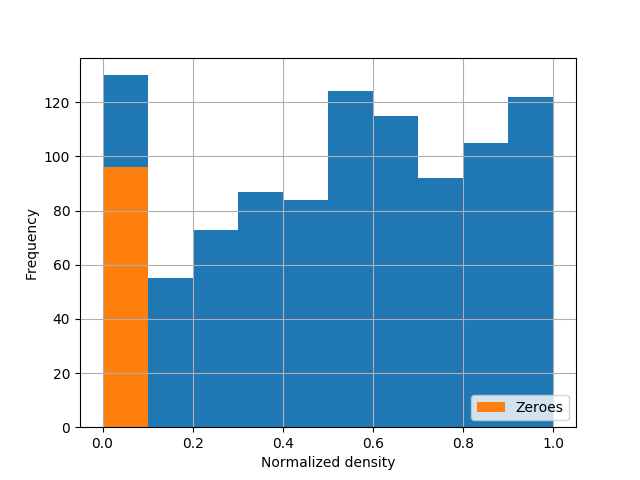
\includegraphics[width=\linewidth]{figures/histogram_normalized_density}
    \caption{Normalized density distribution.}
    \label{fig:hist_normalized_density}
\end{figure}

The normalized density value is low when a class is tested by many tests that only cover a couple of methods, or covered by tests that involve all components.
For example, \texttt{com.google.inject.internal.ProvidesMethodScanner} has 35 branches, i.e. blocks, and its partial spectra is shown in \Cref{tab:providesmethodscanner}.
All the transactions that cover \texttt{Provides\-Method\-Scanner} are sparse, i.e. a row consisting of many zeroes.

\begin{table}[]
\scriptsize
\centering
\caption{Partial activity matrix of the \texttt{com.google.\-inject.\-internal.\-Provides\-Method\-Scanner} class.}
\label{tab:providesmethodscanner}
\begin{tabular}{l|ccccccc}
transaction & $c_1$ & \dots & $c_{22}$ & $c_{23}$ & $c_{24}$ & \dots & $c_{35}$ \\ \hline
\texttt{BinderTest\#testUntargettedBinding} & 0 & \dots & 0 & 1 & 0 & \dots & 0 \\
\texttt{BinderTest\#testMissingDependency} & 0 & \dots & 0 & 1 & 0 & \dots & 0 \\
\texttt{BinderTest\#testProviderFromBinder} & 0 & \dots & 0 & 1 & 0 & \dots & 0 \\
\texttt{BinderTest\#testToStringOnBinderApi} & 0 & \dots & 0 & 1 & 0 & \dots & 0 \\
\texttt{BinderTest\#testUserReportedError} & 0 & \dots & 0 & 1 & 0 & \dots & 0 \\
\vdots & \vdots & \vdots & \vdots & \vdots & \vdots & \vdots & \vdots
\end{tabular}
\end{table}

\begin{table}[]
\scriptsize
\centering
\caption{Activity matrix of the \texttt{org.apache.commons.math4.fitting.least\-squares.Circle\-Problem} class. Every transaction hits every component.}
\label{tab:circleproblem}
\begin{tabular}{l|cccc}
transaction & $c_1$ & $c_2$ & \dots & $c_{26}$ \\ \hline
\texttt{LevenbergMarquardtOptimizerTest\#testParameterValidator} & 1 & 1 & \dots & 1 \\
\texttt{LevenbergMarquardtOptimizerTest\#testCircleFitting2} & 1 & 1 & \dots & 1
\end{tabular}
\end{table}

In the partial spectra of \texttt{Provides\-Method\-Scanner}, see \Cref{tab:providesmethodscanner}, the columns represent branches of \texttt{Provides\-Method\-Scanner}.
For example, in the first row, we observe that the transaction \texttt{test\-Untargetted\-Binding} only hits one branch $c_{23}$, indicated by a 1.
Since every transaction is only hitting a few components, the normalized density is low.
In fact, \texttt{Provides\-Method\-Scanner} has 35 components and if a transaction only hits a few components, it results in the activity matrix to be sparse.

In the spectra of \texttt{org.apache.commons.math4.fitting.least\-squares.Circle\-Problem}, shown in \Cref{tab:circleproblem}, we observe a high density; all branches of \texttt{Circle\-Problem} are hit in every single test.
Since the density is high: 1.0, the normalized density is low: 0.0.

Thus, ideally, to obtain a high value for the normalized density, we need a good balance between tests that cover many components and tests that cover a few.
In Commons Math, the \texttt{org.apache.commons.math4.genetics.Elitistic\-List\-Population} class has a normalized density of 0.979.
In its spectra, see \Cref{tab:elitistic}, we observe that there is a good balance between tests that cover a few components and tests that cover most components.
This results in a density close to 0.5 and a normalized density close 1.0.

\begin{table}[]
\scriptsize
\centering
\caption{Activity matrix of \texttt{org.apache.commons.math4.genetics.Elitistic\-List\-Population}.}
\label{tab:elitistic}
\begin{adjustbox}{center}
\begin{tabular}{l|llllllll}
transaction                                                       & $c_1$ & $c_2$ & $c_3$ & $c_4$ & $c_5$ & $c_6$ & $c_7$ & $c_8$ \\ \hline
\texttt{ElitisticListPopulationTest\#testChromosomeListConstructorTooLow}  & 1     & 0     & 0     & 1     & 0     & 0     & 0     & 0     \\
\texttt{ElitisticListPopulationTest\#testSetElitismRateTooLow}             & 1     & 0     & 0     & 1     & 0     & 0     & 1     & 0     \\
\texttt{ElitisticListPopulationTest\#testConstructorTooHigh}               & 1     & 0     & 0     & 1     & 0     & 0     & 0     & 0     \\
\texttt{ElitisticListPopulationTest\#testConstructorTooLow}                & 1     & 0     & 0     & 1     & 0     & 0     & 0     & 0     \\
\texttt{ElitisticListPopulationTest\#testSetElitismRateTooHigh}            & 1     & 0     & 0     & 1     & 0     & 0     & 1     & 0     \\
\texttt{ElitisticListPopulationTest\#testChromosomeListConstructorTooHigh} & 1     & 0     & 0     & 1     & 0     & 0     & 0     & 0     \\
\texttt{ElitisticListPopulationTest\#testSetElitismRate}                   & 1     & 0     & 0     & 0     & 0     & 1     & 1     & 0     \\
\texttt{ElitisticListPopulationTest\#testNextGeneration}                   & 1     & 1     & 1     & 0     & 1     & 1     & 1     & 1     \\
\texttt{FitnessCachingTest\#testFitnessCaching}                            & 1     & 1     & 1     & 0     & 1     & 1     & 1     & 1     \\
\texttt{GeneticAlgorithmTestBinary\#test}                                  & 1     & 1     & 1     & 0     & 1     & 1     & 1     & 1     \\
\texttt{GeneticAlgorithmTestPermutations\#test}                            & 1     & 1     & 1     & 0     & 1     & 1     & 1     & 1     \\
\texttt{TournamentSelectionTest\#testSelect}                               & 1     & 0     & 0     & 0     & 0     & 0     & 1     & 0
\end{tabular}
\end{adjustbox}
\end{table}

% In short, to obtain a good value for normalized density, a test suite should have a good balance between tests that cover a few components and tests that cover many components.

\section{Diversity}
In \Cref{fig:histogram_diversity}, the distribution of diversity of classes is shown.
The average is 0.588.
The peak for the interval [0, 0.1] occurs for various reasons.
The first reason is that there are classes with only one method and therefore every row is identical, resulting in a diversity of 0.
The second reason is that for some classes there exist only one test case, and in the current Python script the diversity defaults to 0 when there is only one test case.
The third reason is that there are class test suites where all the test cases have identical activity patterns.

\begin{figure}
    \centering
    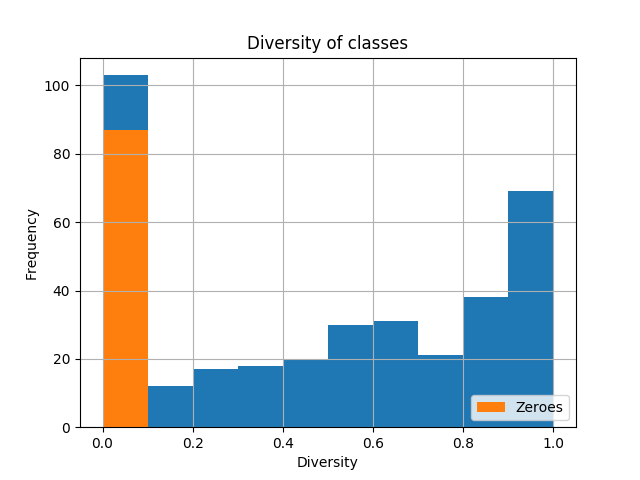
\includegraphics[width=\linewidth]{figures/histogram_diversity}
    \caption{Diversity distribution.}
    \label{fig:histogram_diversity}
\end{figure}

Intuitively, the diversity has a low value when the number of identical transactions, i.e. identical rows in the activity matrix, is high.
Conversely, the diversity is high when the number of identical transactions is low.

\begin{table}[]
\scriptsize
\centering
\caption{Partial activity matrix of \texttt{org.apache.commons.math4.analysis.function.Power}.}
\label{tab:power}
\begin{tabular}{l|ccc}
transaction & $c_1$ & $c_2$ & $c_3$ \\ \hline
\texttt{FunctionUtilsTest\#testFixingArguments} & 1 & 1 & 0 \\
\texttt{FunctionUtilsTest\#testMultiplyDifferentiable} & 1 & 0 & 1 \\
\texttt{FunctionUtilsTest\#testComposeDifferentiable} & 1 & 1 & 1 \\
\texttt{FunctionUtilsTest\#testCompose} & 1 & 1 & 0 \\
\texttt{FunctionUtilsTest\#testMultiply} & 1 & 1 & 0 \\
\texttt{ArrayRealVectorTest\#testMap} & 1 & 1 & 0 \\
\texttt{ArrayRealVectorTest\#testMapToSelf} & 1 & 1 & 0 \\
\texttt{RealVectorTest\#testMap} & 1 & 1 & 0 \\
\vdots & \vdots & \vdots & \vdots
\end{tabular}
\end{table}

In the partial spectra of \texttt{Power}, shown in \Cref{tab:power}, we observe that almost every transaction has an identical activity and therefore the diversity is low: 0.077.
Another reason for the low diversity of \texttt{Power} is that it is covered by 102 test cases, while there are only $2^2 - 1 = 3$ possible different tests for two components.
After 3 unique test cases every additional test will have a negative effect on the diversity because it will share an identical activity with an existing test.

\begin{table}[]
\scriptsize
\centering
\caption{Activity matrix of \texttt{org.apache.commons.math4.ode.AbstractParameterizable}.}
\label{tab:abstractparameter}
\begin{adjustbox}{center}
\begin{tabular}{l|cccccccc}
 & $c_1$ & $c_2$ & $c_3$ & $c_4$ & $c_5$ & $c_6$ & $c_7$ & $c_8$ \\ \hline
\texttt{JacobianMatricesTest\#testHighAccuracyExternalDifferentiation} & 1 & 0 & 1 & 0 & 1 & 0 & 1 & 0 \\
\texttt{JacobianMatricesTest\#testAnalyticalDifferentiation} & 1 & 0 & 1 & 0 & 1 & 0 & 1 & 0 \\
\texttt{JacobianMatricesTest\#testInternalDifferentiation} & 0 & 0 & 0 & 0 & 1 & 0 & 1 & 0 \\
\texttt{JacobianMatricesTest\#testParameterizable} & 1 & 0 & 0 & 0 & 1 & 0 & 1 & 1 \\
\texttt{JacobianMatricesTest\#testWrongParameterName} & 0 & 0 & 1 & 1 & 1 & 1 & 0 & 1 \\
\texttt{JacobianMatricesTest\#testFinalResult} & 1 & 0 & 1 & 0 & 1 & 0 & 1 & 1
\end{tabular}
\end{adjustbox}
\end{table}

In the activity matrix of \texttt{org.\-apache.\-commons.\-math4.\-ode.\-Abstract\-Parameterizable}, shown in \Cref{tab:abstractparameter}, we observe that almost every transaction has a unique activity and therefore its diversity is high: 0.933.
Note that the diversity suffers when there are too many test cases, but does not suffer from a low number of test cases.

An interesting case for diversity is parameterized testing.
Although parameterized is a common practice to test different inputs for a unit, it has a negative effect on the diversity due to identical activity patterns.

\section{Uniqueness}

The distribution of uniqueness of classes is shown in \Cref{fig:uniqueness}.
The average is 0.477.
The peak for the interval [0.9, 1.0] is partially caused by classes that only have one component; activity matrices that consist of one component always have a uniqueness of 1.0.
There are 130 classes that have a uniqueness of 1.0 and 43 out of the 130 classes only have one component.

\begin{figure}
    \centering
    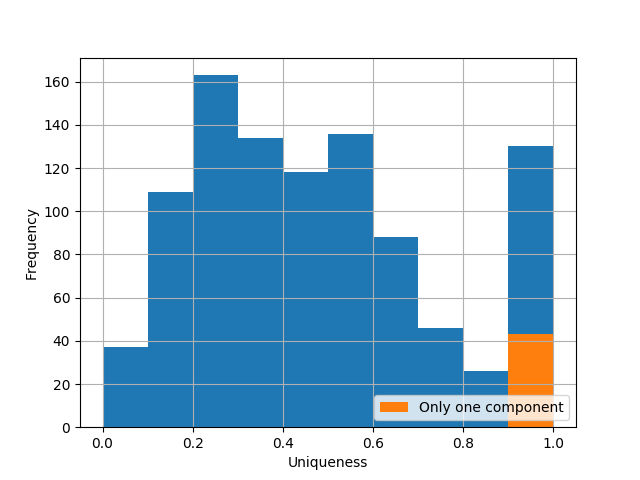
\includegraphics[width=\linewidth]{figures/histogram_uniqueness}
    \caption{Distribution of uniqueness.}
    \label{fig:uniqueness}
\end{figure}

The uniqueness of a class is high when there is a high number of unique columns in the activity matrix.
Conversely, the uniqueness is low when there is a low number of unique columns in the activity matrix.

\begin{table}[]
\scriptsize
\centering
\caption{Activity matrix of \texttt{org.apache.commons.codec.digest.Crypt}.}
\label{tab:crypt}
\begin{adjustbox}{center}
\begin{tabular}{l|cccccccccccc}
 & $c_1$ & $c_2$ & $c_3$ & $c_4$ & $c_5$ & $c_6$ & $c_7$ & $c_8$ & $c_9$ & $c_{10}$ & $c_{11}$ & $c_{12}$ \\ \hline
\texttt{CryptTest\#testDefaultCryptVariant} & 0 & 0 & 0 & 1 & 1 & 0 & 0 & 1 & 0 & 1 & 0 & 0 \\
\texttt{CryptTest\#testCryptWithEmptySalt} & 1 & 1 & 0 & 0 & 0 & 0 & 1 & 1 & 0 & 1 & 1 & 0 \\
\texttt{CryptTest\#testCryptWithBytes} & 0 & 1 & 1 & 1 & 0 & 1 & 0 & 1 & 0 & 1 & 0 & 0 \\
\texttt{Md5CryptTest\#testMd5CryptBytes} & 0 & 1 & 0 & 0 & 0 & 0 & 1 & 1 & 1 & 1 & 1 & 0 \\
\texttt{Md5CryptTest\#testMd5CryptLongInput} & 0 & 1 & 0 & 0 & 0 & 0 & 1 & 1 & 1 & 1 & 1 & 0 \\
\texttt{Md5CryptTest\#testMd5CryptStrings} & 0 & 1 & 0 & 0 & 0 & 0 & 1 & 1 & 1 & 1 & 1 & 0 \\
\texttt{Sha256CryptTest\#testSha256CryptBytes} & 0 & 1 & 0 & 0 & 0 & 0 & 0 & 1 & 0 & 1 & 1 & 1 \\
\texttt{Sha256CryptTest\#testSha256CryptStrings} & 0 & 1 & 0 & 0 & 0 & 0 & 0 & 1 & 0 & 1 & 1 & 1 \\
\texttt{Sha512CryptTest\#testSha512CryptBytes} & 0 & 1 & 1 & 0 & 0 & 0 & 0 & 1 & 0 & 1 & 0 & 0 \\
\texttt{Sha512CryptTest\#testSha512CryptStrings} & 0 & 1 & 1 & 0 & 0 & 0 & 0 & 1 & 0 & 1 & 0 & 0 \\
\texttt{UnixCryptTest\#testUnixCryptStrings} & 1 & 1 & 0 & 0 & 0 & 0 & 1 & 1 & 0 & 1 & 1 & 0 \\
\texttt{UnixCryptTest\#testUnixCryptBytes} & 1 & 1 & 0 & 0 & 0 & 0 & 1 & 1 & 0 & 1 & 1 & 0
\end{tabular}
\end{adjustbox}
\end{table}

An example of a class with a high uniqueness is the \texttt{Crypt} class of Commons Codec, see \Cref{tab:crypt}.
The \texttt{Crypt} class has a uniqueness of 0.916 because it only has one ambiguity group $\langle c_8, c_{10} \rangle$.

\begin{table}[]
\scriptsize
\centering
\caption{Partial activity matrix of \texttt{org.\-apache.\-commons.\-math4.\-random.\-Unit\-Sphere\-Random\-Vector\-Generator}.}
\label{tab:unitsphere}
\begin{tabular}{l|ccccccc}
 & $c_1$ & $c_2$ & $c_3$ & $c_4$ & $c_5$ & $c_6$ & $c_7$ \\ \hline
\texttt{MicrosphereProjectionInterpolatorTest\#testLinearFunction2D} & 1 & 1 & 1 & 1 & 1 & 1 & 1 \\
\texttt{FieldRotationDfpTest\#testDoubleVectors} & 1 & 1 & 1 & 1 & 1 & 1 & 1 \\
\texttt{FieldRotationDfpTest\#testDoubleRotations} & 1 & 1 & 1 & 1 & 1 & 1 & 1 \\
\texttt{FieldRotationDSTest\#testDoubleVectors} & 1 & 1 & 1 & 1 & 1 & 1 & 1 \\
\texttt{FieldRotationDSTest\#testDoubleRotations} & 1 & 1 & 1 & 1 & 1 & 1 & 1 \\
\texttt{SphereGeneratorTest\#testRandom} & 1 & 1 & 1 & 1 & 1 & 1 & 1 \\
\vdots & \vdots & \vdots & \vdots & \vdots & \vdots & \vdots & \vdots
\end{tabular}
\end{table}

In the spectra of \texttt{Unit\-Sphere\-Random\-Vector\-Generator}, see \Cref{tab:unitsphere}, we observe that all components have identical activity patterns and, therefore, the uniqueness is low: 0.142.
Note that the uniqueness does not equal zero although there is no component with a unique activity.

\section{DDU}

The distribution of DDU of classes is shown in \Cref{fig:ddu}.
The average is 0.157.
We observe that 176 classes have a DDU of zero due to normalized density, diversity, or uniqueness being equal to zero.

\begin{figure}
    \centering
    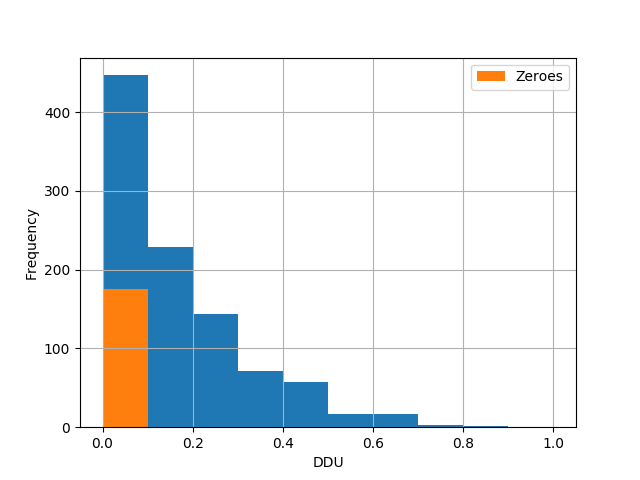
\includegraphics[width=\linewidth]{figures/histogram_ddu}
    \caption{DDU distribution.}
    \label{fig:ddu}
\end{figure}


\begin{table}[]
\scriptsize
\centering
\caption{Activity matrix of \texttt{org.apache.commons.math4.analysis.function.Min}, $\rho' = 1.0$, $\mathcal{G} = 0.809$, and $\mathcal{U} = 1.0$.}
\label{tab:min}
\begin{tabular}{l|cccc}
transaction & $c_1$ & $c_2$ & $c_3$ & $c_4$ \\ \hline
\texttt{UnivariateDifferentiableFunctionTest\#testMinus} & 1 & 0 & 1 & 1 \\
\texttt{FunctionUtilsTest\#testCollector} & 0 & 1 & 0 & 0 \\
\texttt{FunctionUtilsTest\#testAdd} & 1 & 0 & 1 & 0 \\
\texttt{FunctionUtilsTest\#testComposeDifferentiable} & 0 & 0 & 1 & 1 \\
\texttt{FunctionUtilsTest\#testCombine} & 1 & 0 & 1 & 0 \\
\texttt{FunctionUtilsTest\#testCompose} & 1 & 0 & 1 & 0 \\
\texttt{FunctionUtilsTest\#testAddDifferentiable} & 0 & 0 & 1 & 1
\end{tabular}
\end{table}

In \Cref{tab:min}, we observe a class with a high DDU: 0.809.
Its DDU is high because it has an optimal normalized density, uniqueness, and an almost optimal diversity.

\begin{table}[]
\scriptsize
\centering
\caption{Partial activity matrix of \texttt{org.jsoup.parser.ParseSettings}, $\rho' = 0.727$, $\mathcal{G} = 0.204$, and $\mathcal{U} = 0.555$.}
\label{tab:parsesettings}
\begin{tabular}{l|ccccccccc}
transaction & $c_1$ & $c_2$ & $c_3$ & $c_4$ & $c_5$ & $c_6$ & $c_7$ & $c_8$ & $c_9$ \\ \hline
\texttt{ParseTest\#testBaidu} & 0 & 1 & 1 & 0 & 0 & 1 & 1 & 1 & 1 \\
\texttt{AttributesTest\#html} & 0 & 0 & 1 & 0 & 0 & 0 & 1 & 1 & 0 \\
\texttt{HtmlParserTest\#canPreserveAttributeCase} & 0 & 1 & 1 & 0 & 0 & 0 & 1 & 1 & 1 \\
\texttt{HtmlParserTest\#handlesBaseTags} & 0 & 1 & 1 & 0 & 0 & 1 & 1 & 1 & 1 \\
\texttt{SelectorTest\#descendant} & 0 & 1 & 1 & 0 & 0 & 1 & 1 & 1 & 1 \\
\vdots & \vdots & \vdots & \vdots & \vdots & \vdots & \vdots & \vdots & \vdots & \vdots
\end{tabular}
\end{table}

In \Cref{tab:parsesettings}, we observe a class with a low DDU: 0.082.
Eventhough the normalized density and uniqueness are above average, the DDU is low due to the low diversity.

\section{Observations}
In this section, we summarize our findings with regards to normalized density, diversity, uniqueness, and DDU.

The optimal normalized density is 1.0 and the optimal density is 0.5.
The density can be used to guide the developer in writing tests.
For example, when the test suite's density is less than 0.5, it is recommended to write tests that cover many components.
Conversely, when the test suite's density is greater than 0.5, it is recommended to write tests that cover a few components.

In \Cref{tab:providesmethodscanner}, we observed that the more components a class has, the greater the impact of a test, that covers a relative small number of components, has on the sparseness of the activity matrix.

In practice, we write tests to account for many corner cases.
From the diagnostic perspective, adding tests, that do not improve the information gain, is useless.
For example, the diversity can be negatively impacted when we write parameterized tests.
Therefore, we pose the question whether we need a metric that penalizes tests that have identical component coverage.

For DDU the density is normalized such that its operating domain is [0, 1].
However, due to the definition of uniqueness, see \Cref{eq:uniqueness}, its domain is actually (0, 1] instead of [0, 1].

We observe in \Cref{fig:ddu}, that the DDU distribution is right-tailed.
This can be explained by the fact that the DDU is the product of normalized density, diversity, and uniqueness, which all operate in the domain [0, 1].

% Multiplying the individual terms might not be the right approach.
%
% Based on the uniqueness observations, it seems that uniqueness at least requires the developer to write tests that cover a few components.



\chapter{DDU vs. Diagnosability}
\label{ch:rq2}
\begin{framed}
\noindent
\textbf{RQ2:} What is the relation between density, diversity, uniqueness, and DDU and diagnosability?
\end{framed}
In prior work Perez \etal \cite{DBLP:conf/icse/PerezAD17} show that optimizing test suite generation with respect to DDU results in better fault diagnosis.
Therefore, in this chapter, we perform experiments to verify the correlation between DDU and diagnosability, that is, answering RQ2.

\section{Experimental Setup}
\label{sec:rq2_experimental_setup}
First, we have to define the subjects of interest that will be used during the experiments.
For the experiments, we use the open source projects Commons Codec, Commons Compress, and Commons Math, which were also used in prior work by Alex \etal \cite{DBLP:conf/icse/PerezAD17}.
In addition, we include the open source projects Guice and Jsoup due to their popularity on GitHub; both roughly have 5000 stars.

To test the correlation between DDU and diagnosability, we generate 10 artificial multiple components faults of cardinality 2 for each class that has at least 8 components, i.e. method branches.
For each generated fault set, we construct an activity matrix.
We determine for each test that exercises the faulty components whether it is failing according to an \emph{oracle quality probability} of 0.75, which was also used in prior work \cite{DBLP:conf/icse/PerezAD17}.
Then, for each generated activity matrix, we use \emph{STACCATO} to generate fault candidates and \emph{BARINEL} to generate a diagnosis report.
Based on the diagnosis report we compute the wasted effort which is a measurement for diagnosability.
To account for randomness of generating fault sets, we repeat this process 10 times.
Note that we do not generate single component faults because in this case the optimal matrix for diagnosability is a diagonal activity matrix, i.e. each component each tested individually by a unit test.
Additionally, \emph{STACCATO} can sometimes take hours or days to generate fault candidates.
Hence, we discard classes when generating fault candidates takes longer than 10 seconds; this resulted in 16 classes being discarded.

\begin{figure}
  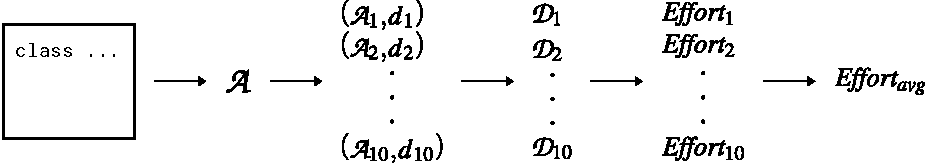
\includegraphics[width=\linewidth]{figures/effort_approach}
  \caption{An activity matrix $\mathcal{A}$ is generated for a particular class. Then, 10 fault candidates of cardinality 2 are generated with a corresponding activity matrix $\mathcal{A}_k$. For each generated matrix, we perform fault diagnosis with \emph{BARINEL} resulting in diagnostic report $\mathcal{D}_k$ and compute the wasted effort. Finally, we compute the average wasted effort. This process is repeated 10 times.}
  \label{fig:fault_generation}
\end{figure}

\begin{figure}
  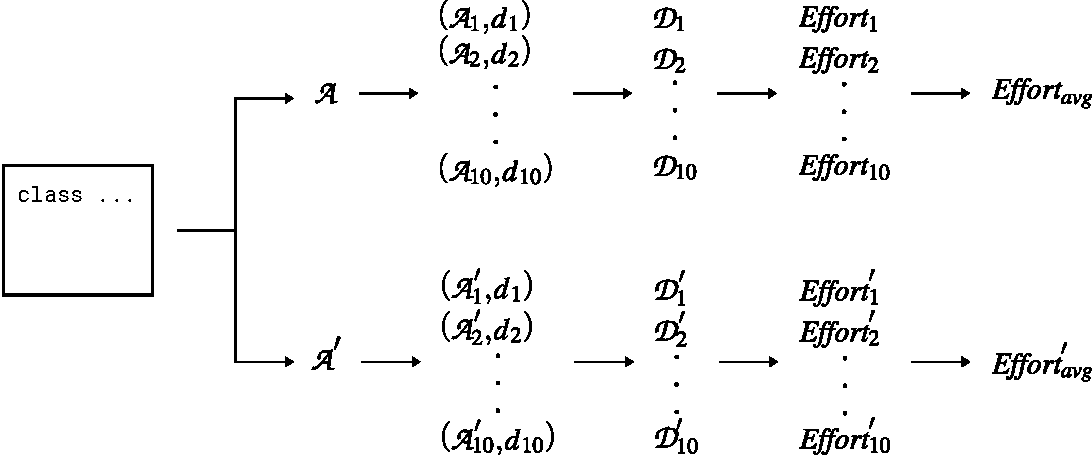
\includegraphics[width=\linewidth]{figures/delta_effort_approach}
  \caption{Two activity matrices $\mathcal{A}$ and $\mathcal{A}'$ are generated for a particular class based on two different test suites. We generate 10 fault candidates of cardinality 2 and accordingly generate 10 activity matrices. Then, we use \emph{BARINEL} to perform fault diagnosis and compute the wasted effort.}
  \label{fig:fault_generation_delta}
\end{figure}

In the construction of the activity matrix we use the branch granularity, that is, every component of the activity matrix represents a method branch; this granularity is also used by Perez \etal \cite{DBLP:conf/icse/PerezAD17}.
To construct the activity matrix of a class we use Perez' DDU Maven plugin\footnote{\url{https://github.com/aperez/ddu-maven-plugin}} using the \texttt{basicblock} granularity, which represents branch granularity.
The steps after the obtaining the activity matrix in \Cref{fig:fault_generation} are performed using Python scripts\footnote{\url{https://github.com/aaronang/ddu}}.

This experiment is different from Perez \etal's work because we do not improve the DDU of a fixed system.
Specifically, in Perez \etal's study, the authors improved the DDU of a fixed system under test by generating new test cases using \emph{EvoSuite}.
However, in this experiment, we compute the DDU for each class and measure for each class its diagnosability using the aforementioned approach.
Essentially, the difference is that we do not improve the DDU of a fixed system but we are simply measuring the DDU.



For this reason, we perform another experiment where we generate two test suites for each class with at least 8 components and at least 10 unit tests.
In addition, we perform the same experiment but for all classes with at least 8 components.
We generate two test suites by using all test cases and 50\% of the test cases.
For both test suites we compute the DDU and randomly generate 10 multiple components faults of cardinality 2 to compute the wasted effort.
Similar to previous experiment we perform this process 10 times to account for randomness of generating fault sets.
The intuition behind this experiment is when we improve the DDU of a fixed system, its diagnosability should improve too.
The setup of this experiment is illustrated in \Cref{fig:fault_generation_delta}.

\section{Experimental Results}
\label{sec:rq2_experimental_results}

\begin{figure*}
    \centering
    \begin{subfigure}[b]{0.49\linewidth}
        \centering
        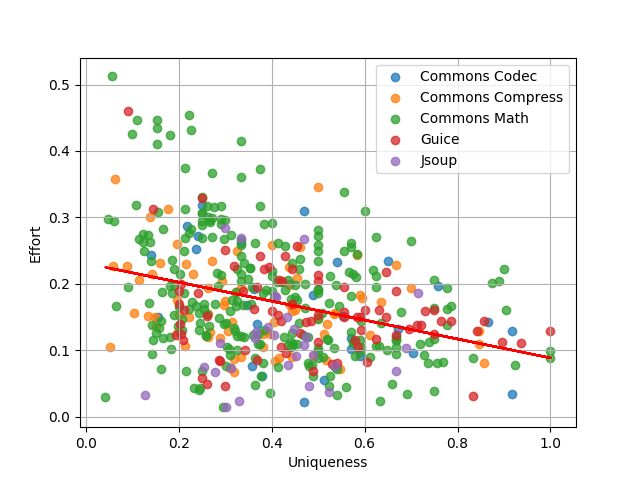
\includegraphics[width=\linewidth]{figures/effort_uniqueness}
        \caption{Uniqueness, $r = -0.120$, $p < 0.001$.}
        \label{fig:effort_uniqueness}
    \end{subfigure}
    \hfill
    \begin{subfigure}[b]{0.49\linewidth}
        \centering
        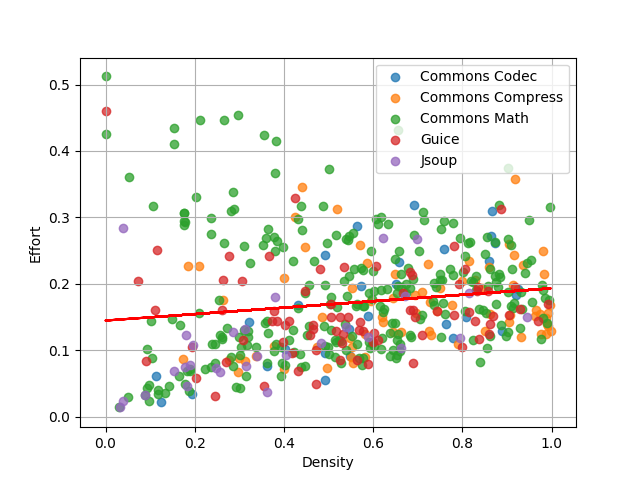
\includegraphics[width=\linewidth]{figures/effort_density}
        \caption{Density, $r = 0.183$, $p < 0.001$.}
        \label{fig:effort_density}
    \end{subfigure}
    \vskip\baselineskip
    \begin{subfigure}[b]{0.49\linewidth}
        \centering
        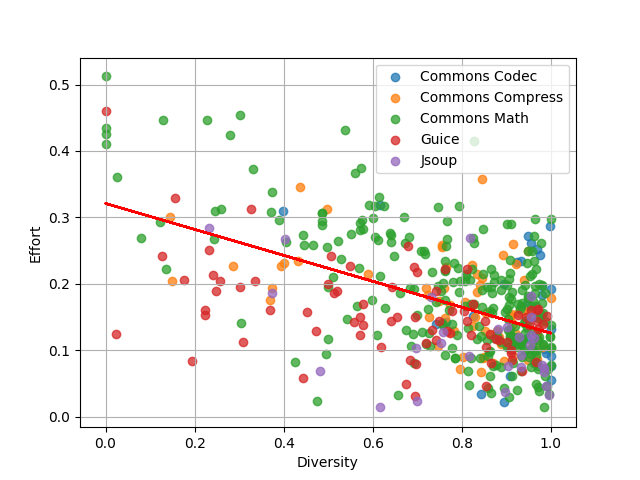
\includegraphics[width=\linewidth]{figures/effort_diversity}
        \caption{Diversity, $r = -0.326$, $p < 0.001$.}
        \label{fig:effort_diversity}
    \end{subfigure}
    \hfill
    \begin{subfigure}[b]{0.49\linewidth}
        \centering
        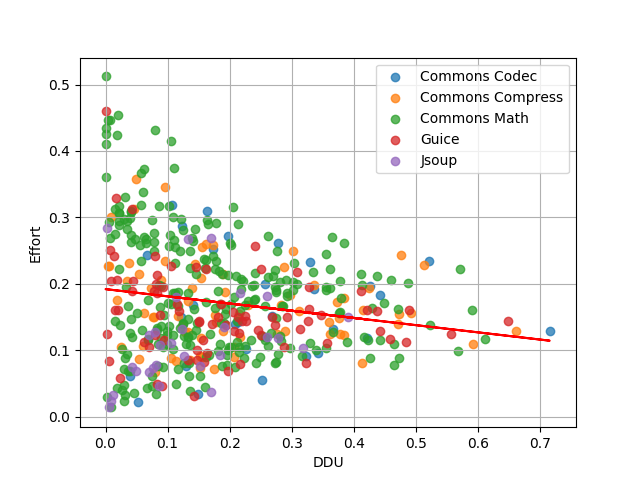
\includegraphics[width=\linewidth]{figures/effort_ddu}
        \caption{DDU, $r = -0.046$, $p = 0.224$.}
        \label{fig:effort_ddu}
    \end{subfigure}
    \caption{Scatterplot of density, diversity, uniqueness, and DDU against effort.}
    \label{fig:metric_vs_effort}
\end{figure*}

In the first experiment, we measure for each class the density, diversity, uniqueness, DDU, and diagnosability.
The results of this experiment are shown in \Cref{fig:metric_vs_effort}.
Note that in \Cref{fig:metric_vs_effort} the population comprises all classes of all projects.
Each datapoint in \Cref{fig:metric_vs_effort} represents a class for which 100 fault candidates are generated in (potentially overlapping) sets of 10 fault candidates as described in \Cref{fig:fault_generation}.
We observe the that there is a positive correlation between density and effort, a negative correlation between diversity and effort, a negative correlation between uniqueness and effort, and a statistically non-significant weak correlation between DDU and effort.

To investigate the relations between these metrics in more detail, we display the correlation values per project in \Cref{tab:correlation_effort}.
For three projects we can say with 95\% confidence that density is correlated with effort.
However, the Pearson correlation for Commons Compress is negative while the Pearson correlation values for Commons Math and Commons Codec are positive.
Hence, the results show no strong evidence that density is correlated with effort.
Regarding diversity and uniqueness, we observe in \Cref{tab:correlation_effort} and \Cref{fig:metric_vs_effort} that both metrics have a weak negative correlation with effort, and that the correlation values in 4 out of 5 projects are statistically significant.
Regarding DDU, for two projects the results show statistical significance that DDU is negatively correlated to effort.
However, for three projects there is no evidence that DDU is correlated to effort.
Therefore, there is no strong evidence that DDU is negatively correlated to effort.

\begin{table}[]
\centering
\caption{Correlation between density, diversity, uniqueness, DDU, and effort.}
\label{tab:correlation_effort}
\begin{adjustbox}{center}
\begin{tabular}{llllll}
\toprule
 &  & \multicolumn{4}{c}{Pearson correlation / Correlation p-value} \\ \cline{3-6}
\multirow{-2}{*}{Subject} & \multirow{-2}{*}{Size} & Density & Diversity & Uniqueness & DDU \\
\rowcolor{Gray}
\cellcolor{Gray} & \cellcolor{Gray} & 0.63 & -0.33 & -0.65 & -0.23 \\
\rowcolor{Gray}
\multirow{-2}{*}{\cellcolor{Gray}\begin{tabular}[c]{@{}l@{}}Commons\\ Codec\end{tabular}} & \multirow{-2}{*}{\cellcolor{Gray}34} & $\mathbf{5.880\times10^{-5}}$ & 0.057 & $\mathbf{3.713\times10^{-5}}$ & 0.197 \\
 &  & -0.22 & -0.45 & -0.40 & -0.37 \\
\multirow{-2}{*}{\begin{tabular}[c]{@{}l@{}}Commons\\ Compress\end{tabular}} & \multirow{-2}{*}{104} & $\mathbf{0.027}$ & $\mathbf{1.348\times10^{-6}}$ & $\mathbf{2.083\times10^{-5}}$ & $\mathbf{1.121\times10^{-4}}$ \\
\rowcolor{Gray}
\cellcolor{Gray} & \cellcolor{Gray} & 0.20 & -0.36 & -0.19 & -0.03 \\
\rowcolor{Gray}
\multirow{-2}{*}{\cellcolor{Gray}\begin{tabular}[c]{@{}l@{}}Commons\\ Math\end{tabular}} & \multirow{-2}{*}{\cellcolor{Gray}420} & $\mathbf{4.982\times10^{-5}}$ & $\mathbf{1.782\times10^{-14}}$ & $\mathbf{7.553\times10^{-5}}$ & 0.572 \\
 &  & 0.01 & -0.31 & -0.29 & -0.22 \\
\multirow{-2}{*}{Guice} & \multirow{-2}{*}{94} & 0.935 & $\mathbf{0.002}$ & $\mathbf{0.005}$ & $\mathbf{0.031}$ \\
\rowcolor{Gray}
\cellcolor{Gray} & \cellcolor{Gray} & 0.29 & -0.37 & 0.16 & 0.20 \\
\rowcolor{Gray}
\multirow{-2}{*}{\cellcolor{Gray}Jsoup} & \multirow{-2}{*}{\cellcolor{Gray}37} & 0.085 & $\mathbf{0.024}$ & 0.337 & 0.229\\
\bottomrule
\end{tabular}
\end{adjustbox}
\end{table}

\begin{figure*}
    \centering
    \begin{subfigure}[b]{0.49\linewidth}
        \centering
        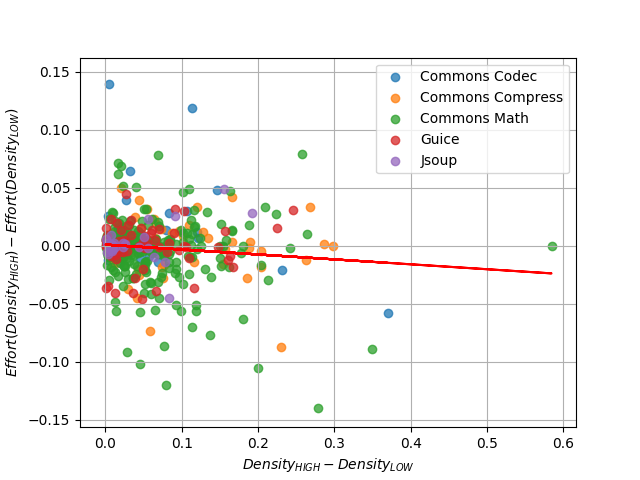
\includegraphics[width=\linewidth]{figures/delta_effort_density}
        \caption{Density, $r=-0.107$, $p<0.01$.}
        \label{fig:delta_effort_density}
    \end{subfigure}
    \hfill
    \begin{subfigure}[b]{0.49\linewidth}
        \centering
        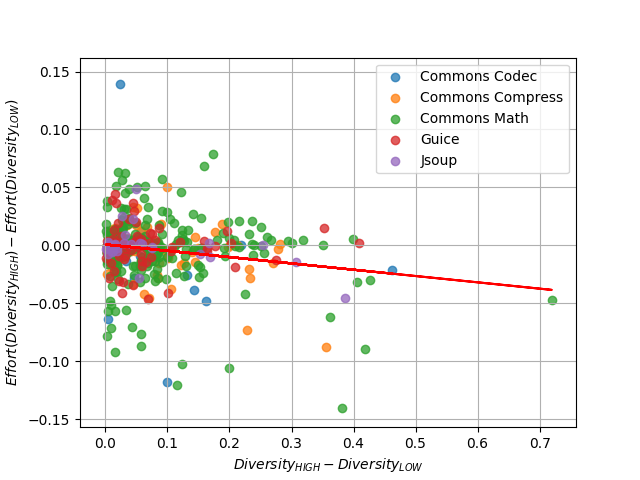
\includegraphics[width=\linewidth]{figures/delta_effort_diversity}
        \caption{Diversity, $r=-0.189$, $p = 4.479\times10^{-5}$.}
        \label{fig:delta_effort_diversity}
    \end{subfigure}
    \vskip\baselineskip
    \begin{subfigure}[b]{0.49\linewidth}
        \centering
        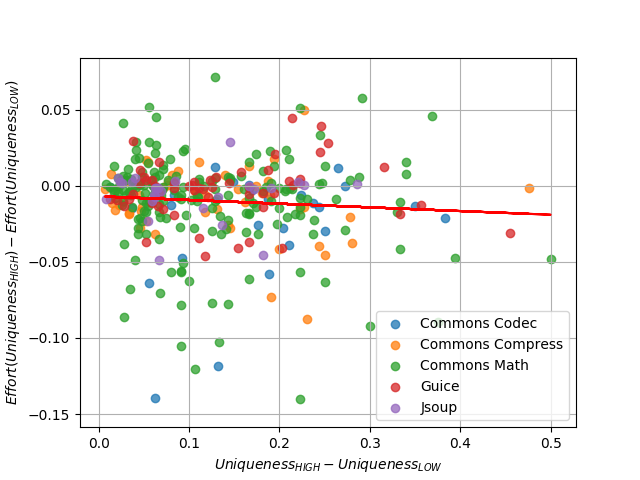
\includegraphics[width=\linewidth]{figures/delta_effort_uniqueness}
        \caption{Uniqueness, $r=-0.079$, $p=0.137$.}
        \label{fig:delta_effort_uniqueness}
    \end{subfigure}
    \hfill
    \begin{subfigure}[b]{0.49\linewidth}
        \centering
        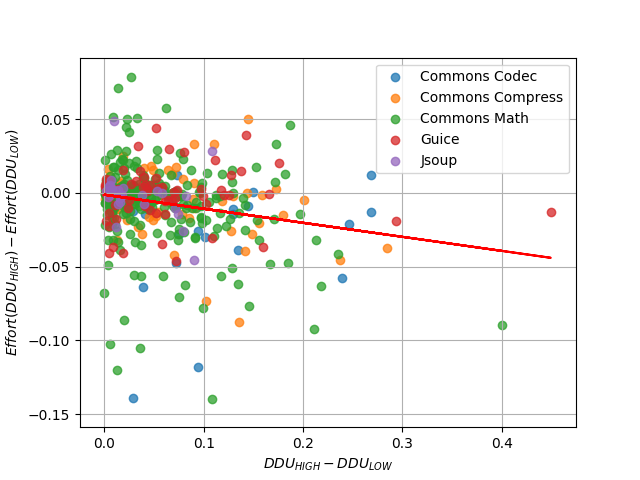
\includegraphics[width=\linewidth]{figures/delta_effort_ddu}
        \caption{DDU, $r=-0.223$, $p=9.044\times10^{-7}$.}
        \label{fig:delta_effort_ddu}
    \end{subfigure}
    \caption{Scatterplot of delta density, delta diversity, delta uniqueness, and delta DDU against delta effort.}
    \label{fig:delta_metric_vs_delta_effort}
\end{figure*}

\begin{table}[]
\centering
\caption{Correlation between delta density, delta diversity, delta uniqueness, delta DDU, and delta effort.}
\label{tab:delta_metric_delta_effort}
\begin{adjustbox}{center}
\begin{tabular}{lllll}
\toprule
 & \multicolumn{4}{c}{Size / Pearson correlation / Correlation p-value} \\
\multirow{-2}{*}{Subject} & Density & Diversity & Uniqueness & DDU \\
\rowcolor{Gray}
\cellcolor{Gray} & 29 & 24 & 26 & 29 \\
\rowcolor{Gray}
\cellcolor{Gray} & -0.277 & -0.229 & 0.230 & 0.011 \\
\rowcolor{Gray}
\multirow{-3}{*}{\cellcolor{Gray}\begin{tabular}[c]{@{}l@{}}Commons\\ Codec\end{tabular}} & 0.145 & 0.281 & 0.256 & 0.950 \\
 & 74 & 73 & 55 & 74 \\
 & -0.098 & -0.372 & -0.217 & -0.297 \\
\multirow{-3}{*}{\begin{tabular}[c]{@{}l@{}}Commons\\ Compress\end{tabular}} & 0.401 & $\mathbf{0.001}$ & 0.111 & $\mathbf{0.010}$ \\
\rowcolor{Gray}
\cellcolor{Gray} & 251 & 256 & 186 & 262 \\
\rowcolor{Gray}
\cellcolor{Gray} & -0.142 & -0.162 & -0.109 & -0.280 \\
\rowcolor{Gray}
\multirow{-3}{*}{\cellcolor{Gray}\begin{tabular}[c]{@{}l@{}}Commons\\ Math\end{tabular}} & $\mathbf{0.023}$ & $\mathbf{0.009}$ & 0.135 & $\mathbf{3.855\times10^{-6}}$ \\
 & 78 & 78 & 57 & 78 \\
 & 0.103 & 0.001 & 0.047 & -0.006 \\
\multirow{-3}{*}{Guice} & 0.368 & 0.995 & 0.728 & 0.952 \\
\rowcolor{Gray}
\cellcolor{Gray} & 29 & 29 & 27 & 29 \\
\rowcolor{Gray}
\cellcolor{Gray} & 0.452 & -0.465 & 0.012 & -0.273 \\
\rowcolor{Gray}
\multirow{-3}{*}{\cellcolor{Gray}Jsoup} & $\mathbf{0.013}$ & $\mathbf{0.011}$ & 0.951 & 0.150\\
\bottomrule
\end{tabular}
\end{adjustbox}
\end{table}

In the second experiment, we generate two test suites for a given class: a test suite with 50\% of the test cases enabled, and a test suite with 100\% of the test cases enabled.
This naturally results in two test suites with two different DDU values.
For each class, we compare the effort of a test suite with a lower DDU value with a test suite with a higher DDU value.
Identical approach is used for density, diversity, and uniqueness.
Note that we exclude classes where the two test suites do not result in a metric difference.
The results of this experiment are shown in \Cref{fig:delta_metric_vs_delta_effort} and \Cref{tab:delta_metric_delta_effort}.
In \Cref{fig:delta_metric_vs_delta_effort}, we observe that an increase in any metric --- density, diversity, uniqueness, DDU --- results in a lower required effort to diagnose mistakes.
Although the results are statistically significant, see \Cref{fig:delta_metric_vs_delta_effort}, the correlations are weak.

Revisiting the second research question:
\begin{framed}
\noindent
\textbf{RQ2:} What is the relation between density, diversity, uniqueness, and DDU and diagnosability?
\end{framed}
\textbf{A:} In the first experiment, two out of the five projects show that DDU is negatively correlated with diagnosability.
In the second experiment, two out of the five projects show that improving the DDU value of a class' test suite will improve the diagnosability.
Therefore, based on these two experiments, there is no evidence that DDU is strongly correlated to diagnosability.
However, in the second experiment, we observe that an increase in DDU is weakly correlated to an decrease in effort and, thus, weakly correlated to diagnosability.
There is also no strong evidence that density, diversity, and uniqueness are correlated to diagnosability.

\chapter{DDU vs. Test Coverage}
\label{ch:rq3}

\begin{framed}
\noindent
\textbf{RQ3:} What is the relation between density, diversity, uniqueness, and DDU and test coverage?
\end{framed}

In this chapter, we investigate the relation between DDU and test coverage.
The reason for researching the relation between DDU and test coverage is to investigate whether DDU should be used as a complementary metric to test coverage as Perez \etal proposed.
If there is a strong correlation between DDU and test coverage, then it means that DDU might function as an error detection metric too.
Furthermore, investigating the relation between DDU and test coverage might give us insight in how DDU and test coverage could work together in practice.

To answer the research question we will perform several experiments.
First, we would like to confirm that test coverage is strongly correlated with error detection since test coverage presumably optimizes the test suite for error detection.
Second, we would like to investigate the relation between DDU and test coverage.
Third, we would like to examine the relation between DDU and error detection.


\section{Experimental Setup}
We have to measure the test coverage and error detection to analyze the relation between test coverage and error detection.
Test coverage can be determined by dividing the number of components hit in the activity matrix by the total number of components in the activity matrix.
Given the acitity matrix in \Cref{tab:test_coverage}, we observe that 3 out of the 4 components are hit and therefore the test coverage is $\frac{3}{4} = 0.75$.
\begin{table}[]
\centering
\caption{Example of activity matrix with a test coverage of 75\%. Bolded components are hit by one of the tests.}
\label{tab:test_coverage}
\begin{tabular}{l|llll}
transactions & $\mathbf{c_1}$ & $\mathbf{c_2}$ & $c_3$ & $\mathbf{c_4}$ \\ \hline
$t_1$ & 0 & 0 & 0 & 1 \\
$t_2$ & 1 & 0 & 0 & 1 \\
$t_3$ & 1 & 1 & 0 & 0
\end{tabular}
\end{table}
The error detection is computed by generating 10 artificial faults --- in the experiments we generate multiple components faults with a cardinality 2.
For each fault, we compute the error vector using an \emph{oracle probability} of 0.75, similar to Perez \etal's study, and check whether the vector contains an error, i.e. $1 \in e_i$.
Finally, the error detection is computed by dividing the sum of faults that were detected by 10, the number of generated faults.
To account for randomness of generating fault candidates, we repeat this process 10 times.
We obtain the activity matrices by using Perez \etal's \texttt{ddu-maven-plugin}, similar to the experiments in \Cref{ch:rq2}.
The computation of error detection is illustrated in \Cref{fig:error_detection_computation}.
\begin{figure}[b]
  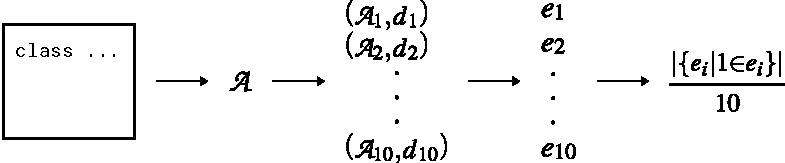
\includegraphics[width=\linewidth]{figures/error_detection}
  \caption{We compute the activity matrix for a given class and generate 10 artificial fault candidates ($d_1$, $d_2$, $d_{10}$) of cardinality 2. For each pair $(\mathcal{A}_i, d_i)$, the error vector $e_i$ is computed. The error detection is computed by dividing the sum of faults that were detected ($|\{e_i | 1 \in e_i \}|$) by 10, the number of generated faults.}
  \label{fig:error_detection_computation}
\end{figure}

For the second experiment, in which we investigate the relation between DDU and test coverage, we compute the normalized density, diversity, uniqueness, DDU, and test coverage for each activity matrix, and compute the correlation.
Furthermore, we use a similar approach as the experiments in \Cref{ch:rq2}, see \Cref{fig:delta_test_coverage_approach}, where we create two test suites: (1) a test suite that consists of 50\% of the available tests and (2) a test suite that consists of 100\% of the available tests.
This will most likely result in a system with two test suites with different DDU values, allowing us to investigate whether improving the DDU for a fixed system results in a test coverage improvement.
\begin{figure}
  \center
  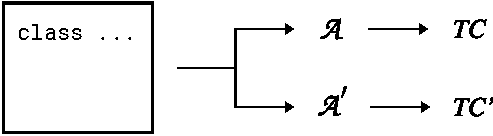
\includegraphics[width=0.6\linewidth]{figures/delta_test_coverage_approach}
  \caption{For each class, two test suites are generated, resulting in two activity matrices $\mathcal{A}$ and $\mathcal{A}'$. For each activity matrix, we compute test coverage $TC$, DDU, normalized density, diversity, uniqueness.}
  \label{fig:delta_test_coverage_approach}
\end{figure}

For the third experiment, we generate two test suites with different DDU values and investigate whether the error detection improves when DDU improves, see \Cref{fig:delta_error_detection_approach}.
Similar to the first experiment, we generate 10 fault candidates of cardinality 2 and compute the error vector with an \emph{oracle probability} of 0.75 to determine the error detection.
To account for randomness of generating fault candidates, we repeat this process 10 times.
\begin{figure}
  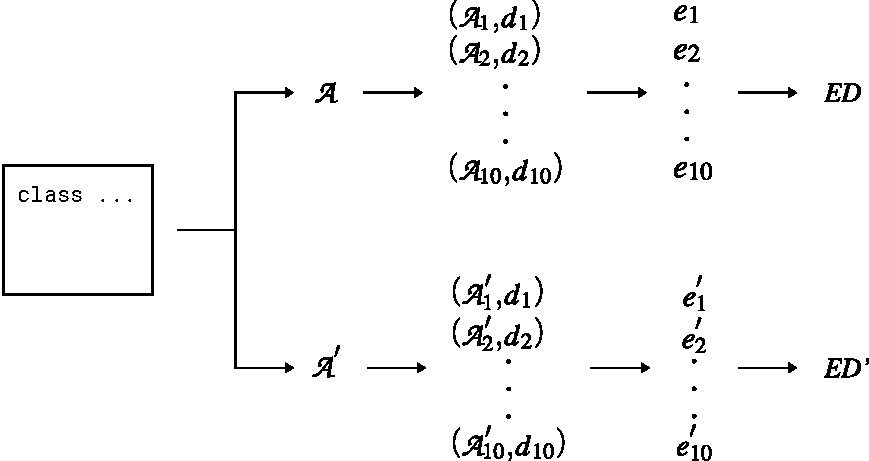
\includegraphics[width=\linewidth]{figures/delta_error_detection_approach}
  \caption{For each class, we generate two different test suites, resulting in a two activity matrices. For each matrix, we generate 10 fault candidates of cardinality 2 and compute the error vector. Finally, we compute the error detection and repeat this process 10 times.}
  \label{fig:delta_error_detection_approach}
\end{figure}

Note that for the experiments we use the same projects as previous ones, namely Commons Codec, Commons Compress, Commons Math, Guice, Jsoup.

\section{Experimental Results}

\todo{First experiment results}
In the first experiment, we confirm that test coverage is representative for error detection.
In \Cref{fig:coverage_error_detection}, we observe that there is a strong correlation between branch coverage and error detection.
It seems that test coverage also puts an upper bound on error detection.



\begin{figure}
  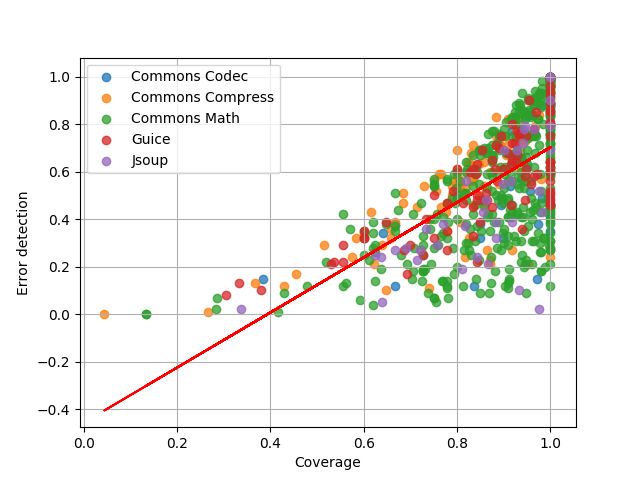
\includegraphics[width=\linewidth]{figures/coverage_error_detection}
  \caption{Scatterplot of coverage and error detection, $r = 0.628$, $p < 0.01$.}
  \label{fig:coverage_error_detection}
\end{figure}

\todo{Second experiment results}

\begin{figure*}
    \centering
    \begin{subfigure}[b]{0.49\linewidth}
        \centering
        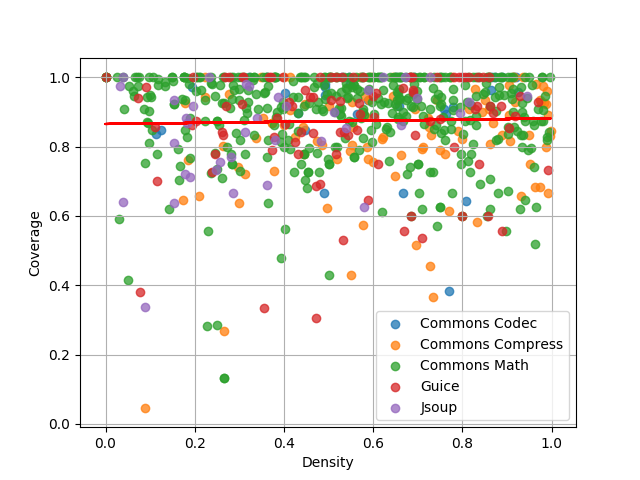
\includegraphics[width=\linewidth]{figures/coverage_density}
        \caption{Density, $r=0.029$, $p = 0.44$.}
        \label{fig:coverage_density}
    \end{subfigure}
    \hfill
    \begin{subfigure}[b]{0.49\linewidth}
        \centering
        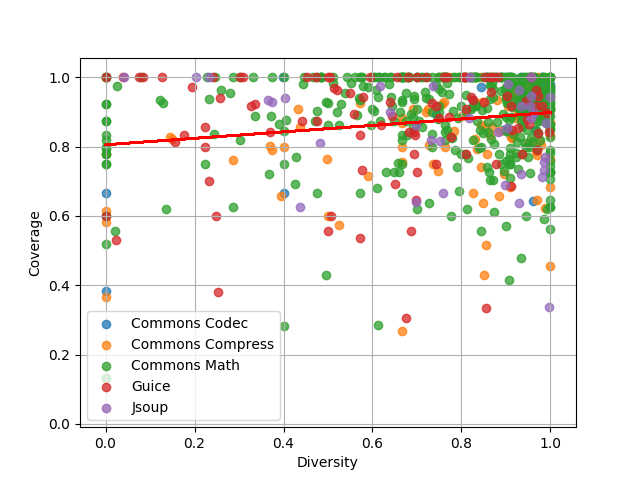
\includegraphics[width=\linewidth]{figures/coverage_diversity}
        \caption{Diversity, $r=0.173$, $p < 0.01$.}
        \label{fig:coverage_diversity}
    \end{subfigure}
    \vskip\baselineskip
    \begin{subfigure}[b]{0.49\linewidth}
        \centering
        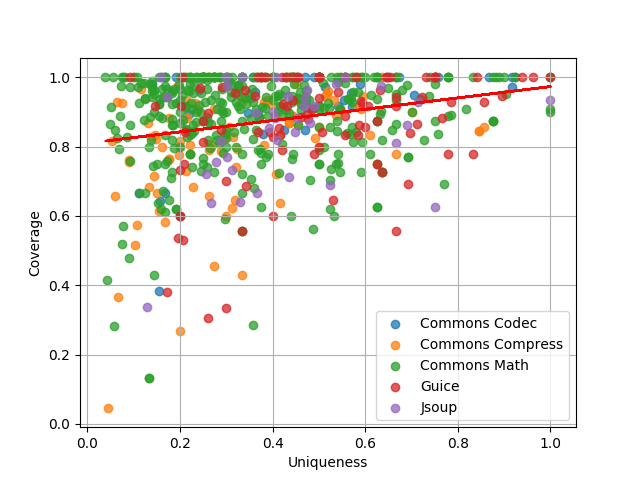
\includegraphics[width=\linewidth]{figures/coverage_uniqueness}
        \caption{Uniqueness, $r=0.237$, $p<0.01$.}
        \label{fig:coverage_uniqueness}
    \end{subfigure}
    \hfill
    \begin{subfigure}[b]{0.49\linewidth}
        \centering
        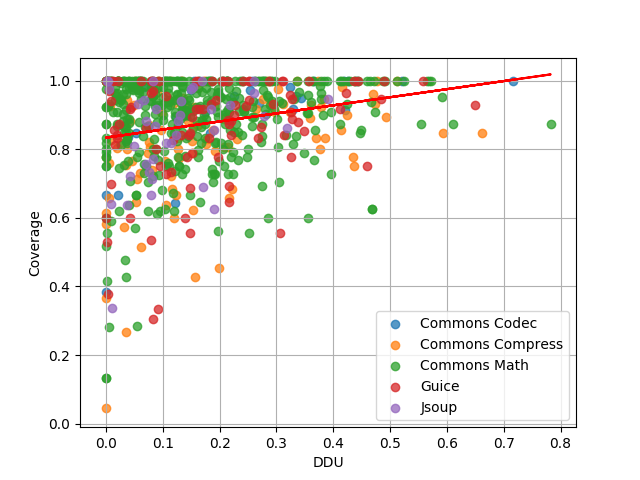
\includegraphics[width=\linewidth]{figures/coverage_ddu}
        \caption{DDU, $r=0.228$, $p<0.01$.}
        \label{fig:coverage_ddu}
    \end{subfigure}
    \caption{Scatterplot of normalized density, diversity, uniqueness, and DDU against branch coverage.}
    \label{fig:coverage_metric}
\end{figure*}

\begin{figure*}
    \centering
    \begin{subfigure}[b]{0.49\linewidth}
        \centering
        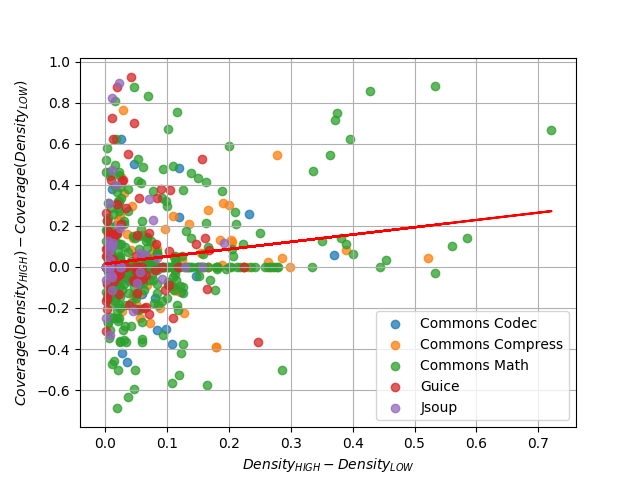
\includegraphics[width=\linewidth]{figures/delta_coverage_density}
        \caption{Density, $r=0.143$, $p<0.01$.}
        \label{fig:delta_coverage_density}
    \end{subfigure}
    \hfill
    \begin{subfigure}[b]{0.49\linewidth}
        \centering
        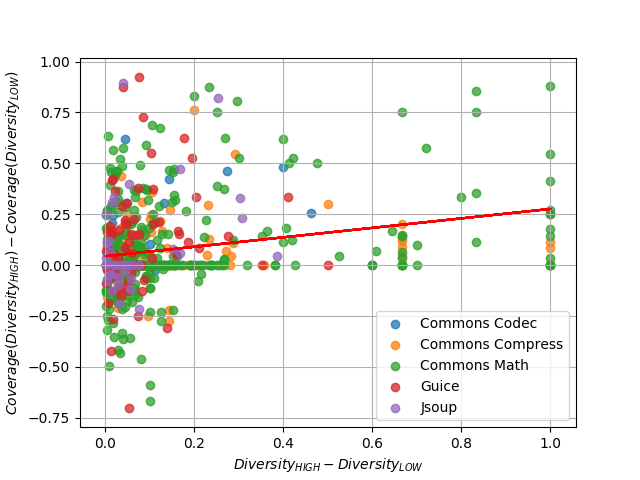
\includegraphics[width=\linewidth]{figures/delta_coverage_diversity}
        \caption{Diversity, $r=0.230$, $p < 0.01$.}
        \label{fig:delta_coverage_diversity}
    \end{subfigure}
    \vskip\baselineskip
    \begin{subfigure}[b]{0.49\linewidth}
        \centering
        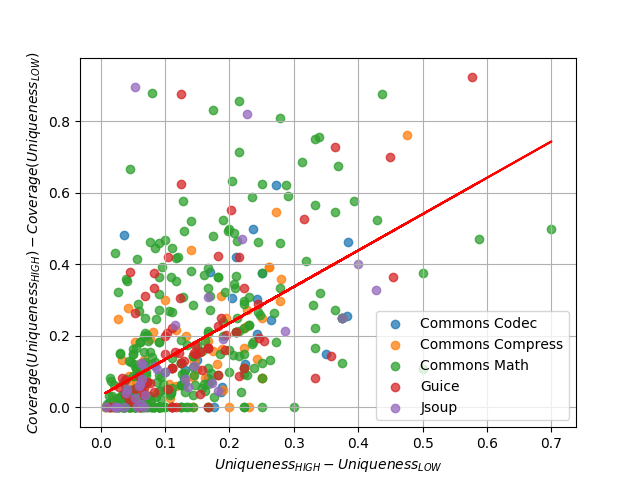
\includegraphics[width=\linewidth]{figures/delta_coverage_uniqueness}
        \caption{Uniqueness, $r=0.546$, $p<0.01$.}
        \label{fig:delta_coverage_uniqueness}
    \end{subfigure}
    \hfill
    \begin{subfigure}[b]{0.49\linewidth}
        \centering
        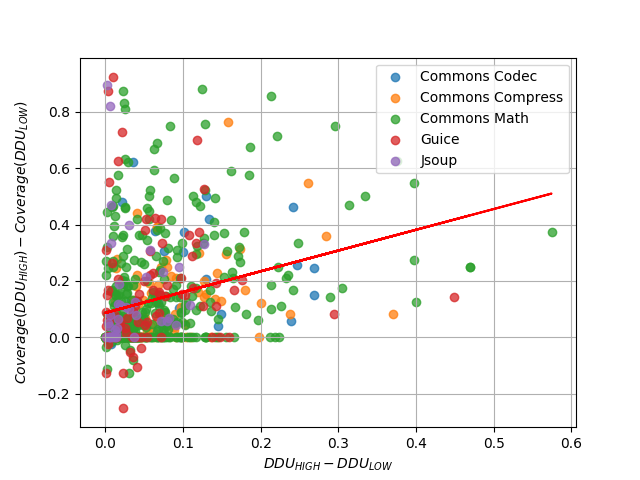
\includegraphics[width=\linewidth]{figures/delta_coverage_ddu}
        \caption{DDU, $r=0.290$, $p<0.01$.}
        \label{fig:delta_coverage_ddu}
    \end{subfigure}
    \caption{Scatterplot of delta normalized density, delta diversity, delta uniqueness, and delta DDU against delta branch coverage.}
    \label{fig:delta_coverage_metric}
\end{figure*}

\todo{Third experiment results}

\begin{figure*}
    \centering
    \begin{subfigure}[b]{0.49\linewidth}
        \centering
        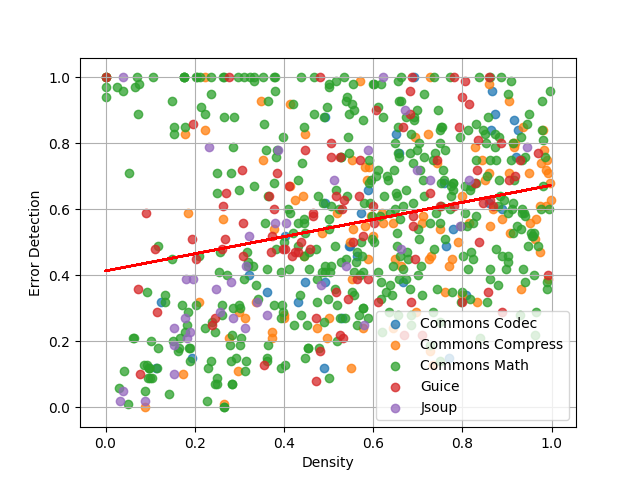
\includegraphics[width=\linewidth]{figures/error_detection_density}
        \caption{Density, $r=0.256$, $p<0.01$.}
        \label{fig:error_detection_density}
    \end{subfigure}
    \hfill
    \begin{subfigure}[b]{0.49\linewidth}
        \centering
        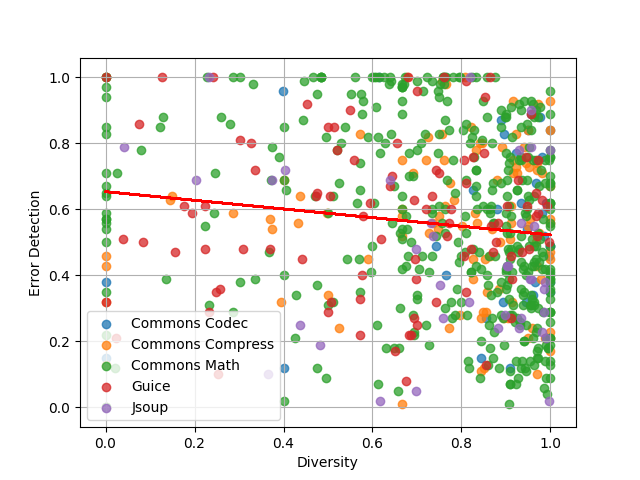
\includegraphics[width=\linewidth]{figures/error_detection_diversity}
        \caption{Diversity, $r=-0.132$, $p < 0.01$.}
        \label{fig:error_detection_diversity}
    \end{subfigure}
    \vskip\baselineskip
    \begin{subfigure}[b]{0.49\linewidth}
        \centering
        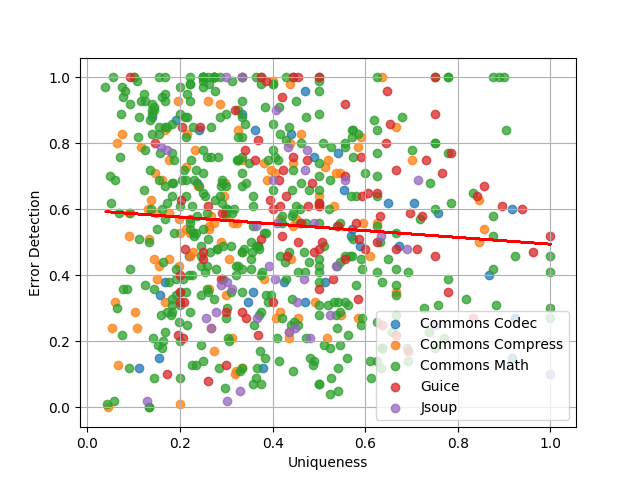
\includegraphics[width=\linewidth]{figures/error_detection_uniqueness}
        \caption{Uniqueness, $r=-0.080$, $p<0.05$.}
        \label{fig:error_detection_uniqueness}
    \end{subfigure}
    \hfill
    \begin{subfigure}[b]{0.49\linewidth}
        \centering
        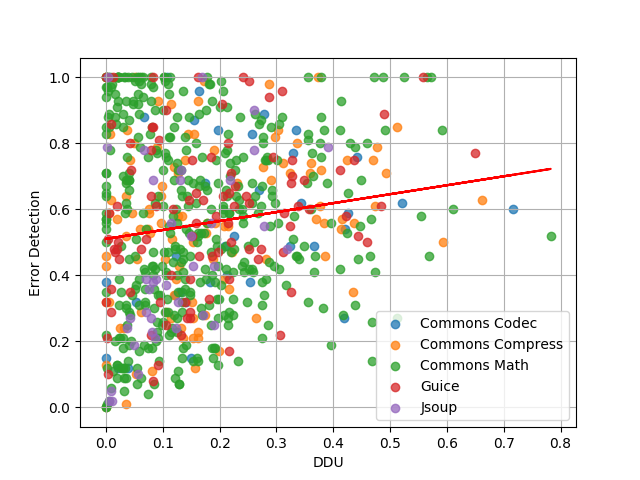
\includegraphics[width=\linewidth]{figures/error_detection_ddu}
        \caption{DDU, $r=0.142$, $p<0.01$.}
        \label{fig:error_detection_ddu}
    \end{subfigure}
    \caption{Scatterplot of normalized density, diversity, uniqueness, and DDU against error detection.}
    \label{fig:error_detection_metric}
\end{figure*}

\begin{figure*}
    \centering
    \begin{subfigure}[b]{0.49\linewidth}
        \centering
        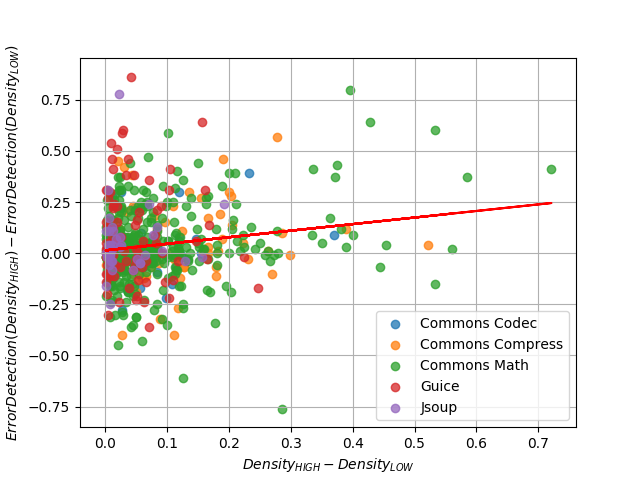
\includegraphics[width=\linewidth]{figures/delta_error_detection_density}
        \caption{Density, $r=0.165$, $p<0.01$.}
        \label{fig:delta_error_detection_density}
    \end{subfigure}
    \hfill
    \begin{subfigure}[b]{0.49\linewidth}
        \centering
        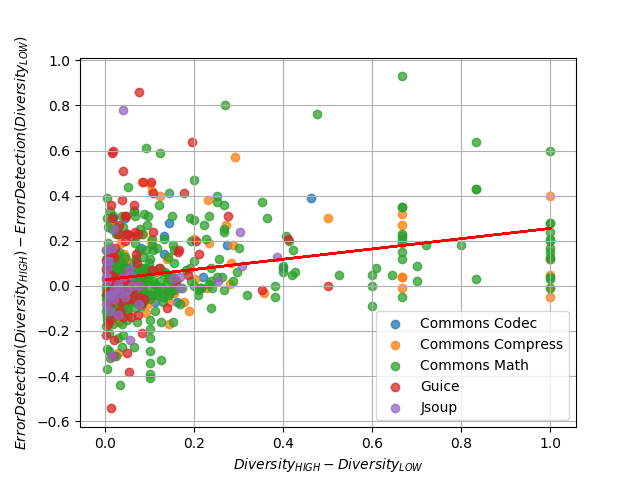
\includegraphics[width=\linewidth]{figures/delta_error_detection_diversity}
        \caption{Diversity, $r=0.275$, $p < 0.01$.}
        \label{fig:delta_error_detection_diversity}
    \end{subfigure}
    \vskip\baselineskip
    \begin{subfigure}[b]{0.49\linewidth}
        \centering
        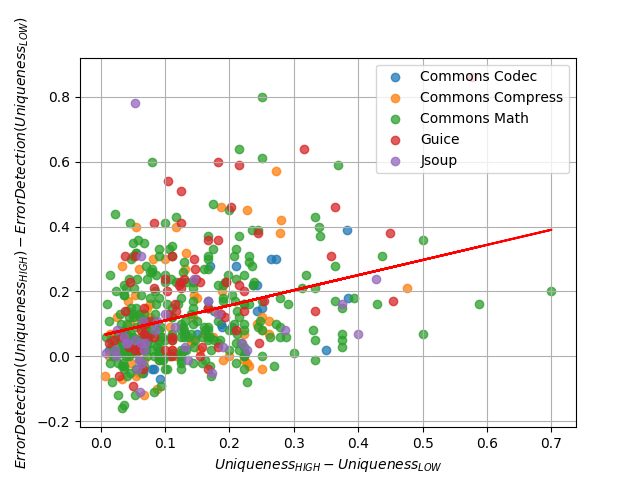
\includegraphics[width=\linewidth]{figures/delta_error_detection_uniqueness}
        \caption{Uniqueness, $r=0.323$, $p<0.01$.}
        \label{fig:delta_error_detection_uniqueness}
    \end{subfigure}
    \hfill
    \begin{subfigure}[b]{0.49\linewidth}
        \centering
        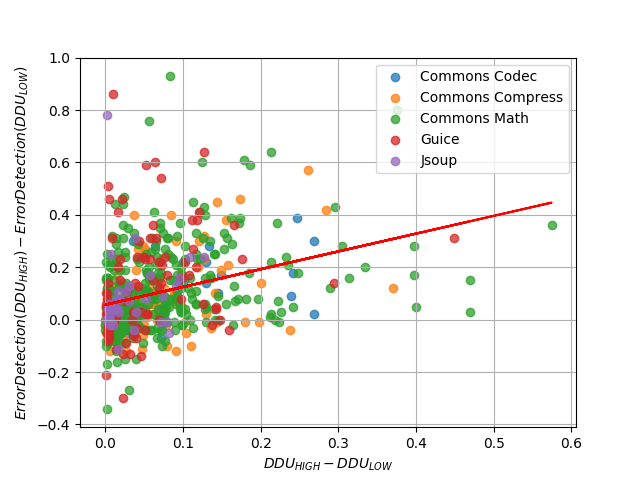
\includegraphics[width=\linewidth]{figures/delta_error_detection_ddu}
        \caption{DDU, $r=0.324$, $p<0.01$.}
        \label{fig:delta_error_detection_ddu}
    \end{subfigure}
    \caption{Scatterplot of delta normalized density, delta diversity, delta uniqueness, and delta DDU against delta error detection.}
    \label{fig:delta_error_detection_metric}
\end{figure*}

\todo{Answer RQ}



% \chapter{Analysis Framework}

\chapter{Improving DDU}

\chapter{Conclusion}
\label{ch:conclusion}


\bibliographystyle{plain}
\bibliography{bibliography}

\end{document}
